\documentclass{article}
\usepackage{cite}
\usepackage[export]{adjustbox}[2011/08/13]
\usepackage[hyphens,spaces,obeyspaces]{url}
\usepackage{amsmath,amssymb,amsfonts}
\usepackage{algorithmic}
\usepackage{graphicx}
\usepackage{subcaption}
\usepackage{textcomp}
\usepackage{xcolor}
\usepackage{csquotes}
\usepackage{listings}

\newcommand\descitem[1]{\item{\bfseries #1}\\}

\begin{document}

\begin{titlepage}

\newcommand{\HRule}{\rule{\linewidth}{0.5mm}} % Defines a new command for the horizontal lines, change thickness here

\center % Center everything on the page
 
%----------------------------------------------------------------------------------------
%	HEADING SECTIONS
%----------------------------------------------------------------------------------------

\textsc{\LARGE University of St Andrews}\\[1.5cm] % Name of your university/college
\textsc{\large CS5199 Final Report}\\[0.5cm] % Minor heading such as course title

%----------------------------------------------------------------------------------------
%	TITLE SECTION
%----------------------------------------------------------------------------------------

\HRule \\[0.4cm]
{ \huge \bfseries A Strategy Video-Game for Collaborative Agents with a Personality and Humoristic Dialogues}\\[0.4cm] % Title of your document
\HRule \\[1.0cm]
 
%----------------------------------------------------------------------------------------
%	AUTHOR SECTION
%----------------------------------------------------------------------------------------

\Large \emph{Author:}\\
 \textsc{Jordan Mackie}\\[1cm] % Your name
\Large \emph{Supervisors:}\\
 \textsc{Dr Alice Toniolo \hspace{0.8cm}}
\textsc{Christopher Stone}\\[0.7cm] % Your name
 
%----------------------------------------------------------------------------------------
%	DATE SECTION
%----------------------------------------------------------------------------------------

{\large \today}\\[1cm] % Date, change the \today to a set date if you want to be precise

%----------------------------------------------------------------------------------------
%	LOGO SECTION
%---------------------------------------------------------------------------------------


\includegraphics[width = 4.3cm]{images/standrewslogo.png}
 
%----------------------------------------------------------------------------------------

\vfill % Fill the rest of the page with whitespace

\end{titlepage}

\section*{Abstract}

We built a system of collaborative agents with personality driven decisions and humoristic dialogues with the goal of providing entertainment and also providing a human friendly way of interpreting agent interactions in multiagent systems. The agents were designed to play chess, each representing a single piece, and given goal-based personalities that would affect their decisions and how they would interact with other agents. We gathered feedback through allowing volunteers to play against our agents and asking questions covering usability and enjoyment. Finally, we present our results and discuss further work or areas of improvement that could be taken up.

\section*{Declaration}

I declare that the material submitted for
assessment is my own work except where credit is
explicitly given to others by citation or
acknowledgement. This work was performed during
the current academic year except where otherwise
stated.
The main text of this project report is %TODO NN,NNN*
words long, including project specification and plan.
In submitting this project report to the University of
St Andrews, I give permission for it to be made
available for use in accordance with the regulations of
the University Library. I also give permission for
the title and abstract to be published and for copies of
the report to be made and supplied at cost to any bona
fide library or research worker, and to be made
available on the World Wide Web. I retain the
copyright in this work.

\clearpage

\tableofcontents

\clearpage

\section{Introduction}

Multiagent systems are the next step to increase the level of autonomy that can be provided by technology. Agents that are able to learn, adapt, and negotiate with other agents to achieve their goals allow for complex problems to be solved or modelled without human intervention, such as monitoring and maintaining national power grids \cite{archon}. 

Often, developers and users will anthropomorphise these agents when describing their behaviour. This project aimed to encourage this by implementing agents with a model of personality that affects their choice of actions, by rendering the negotiations between agents in a natural language, and by using models of humour to make the interactions between agents entertaining. 

There is currently a great deal of research in improving conversational agents for human interaction, but little work in agent to agent interaction. As we discuss later, this work would be beneficial for game development by emulating realistic interactions in the world around the player. There are also possible applications in robotics and digital assistants. 

Therefore, our main goal was to create a model of personalities that would be able to select actions for each agent, and to also reflect these personalities and the actions taken in the form of natural language. This would require what we later refer to as a conversation planner, a natural language generation system for mapping these actions to statements in English, and a system for determining which next actions were available and of these actions which would be preferred by an agents personality.

In order to present these features in a user friendly manner, we also had to design and implement a system composed of a graphical interface for the user and a server that would maintain the life cycle of the game and all the agents involved in the game. 

Chess was chosen as our strategy game as multiagent implementations have been previously investigated, though not in a configuration where agents could have conflicting goals in the same team. However, our model for determining agent actions can be applied to any other strategy game or multiagent system.

We evaluated our system to determine how effective it was as a chess engine by scoring its moves using the open-source chess AI, Stockfish \cite{stockfish}. We also carried out our own assessment of the conversations and natural language generation features. Finally we also gathered user feedback from a group of participants, who after being presented videos of gameplay and given a chance to play against the agents themselves completed a questionnaire. The results of this questionnaire were analysed to allow us to identify the parts of the project that were successful and the parts that required further work.

Due to time constraints and the wide range of complex problems being solved, we were not able to perfect each feature. However, our user feedback and personal evaluation of the final artefact suggested that our implementation was successful. Users were entertained by the discussions between agents and their reactions to events during the game, and many were keen to continue even outside of the feedback exercise. Though our strategic evaluation showed that as a chess AI, our agents were not particularly effective, the conversational planner and personality features which were the main problems we had hoped to tackle were well received.

\section{Context Survey}

\subsection{Multiagent Systems in Entertainment}

Many modern video games involve the user managing multiple characters to achieve some goal, such as producing in-game resources or defending against an opponent. This sort of problem lends itself easily to multiagent systems. Instead of having one artificial intelligence engine driving the actions of all the characters, developers can create agents with a limited set of actions and some concept of progress towards their goals and allow emergent behaviour to find a solution to the problem, sometimes in surprising ways. 

Ocio and Brugos \cite{sandboxmas} discuss how multiagent systems can be applied to create more realistic worlds in sandbox games. By implementing the environment, objects, and non-playable characters (NPCs) as agents, developers can create a world that reacts and adapts the player, but also operates in isolation from the character to provide a realistic setting. The concept of personalities is also mentioned as a way of allowing similar NPCs to exhibit different slightly different behaviours, such as having aggressive or relaxed driving styles.

Even in games with very simple rules and logic, multiagent systems can find interesting and complex solutions. OpenAI implemented hide-and-seek using agents, where hiders avoid the line-of-sight of the seekers \cite{openaiemergent}. The game was played in a world with randomly generated walls and objects such as ramps (for climbing over walls) and blocks (for forming barricades). What made this fascinating is that the agents were not incentivised to use these objects, but after repeatedly playing and learning, both the hiders and seekers created strategies such as blocking each other in a safe area, and even removing the objects from the other team before hiding.

Knowing that multi-agent autocurricula can realise strategies not considered by humans, \cite{masboardgames} discuss how they can be applied to strategy board games such as Diplomacy and Risk. They describe a generic framework for supporting agent-based competitive bots for board games and then implement bots for the aforementioned games. Their research suggests that for games with a large number of units and a large action space, a multi-agent approach can identify effective strategies quicker than the exhaustive methods used for chess engines. 

\subsection{Multiagent System Frameworks}

Most multiagent systems have similar requirements, and so several frameworks have been developed to bootstrap their development. \cite{massurvey} provide a very thorough survey of the frameworks currently in use today and highlight various features and drawbacks in their implementation. 

The most popular is the Java Agent Development Framework (JADE) \cite{jade}. It conforms to the FIPA standard, which is a protocol for agent communication that involves defining performatives (e.g. request, inform), language name, and other message meta-data during communication. The benefit of systems that abide this standard is that they are able to interact regardless of the technology used to implement them. JADE provides other important features such as base classes for agent functionality called behaviours, a directory facilitator (DF) agent implementation to allow agents to find each other, and an Agent Management Service that manages and tracks the lifecycle of agents and allows them to move between containers (which can exist on multiple hosts). To aid during development, JADE also incldues a GUI for debugging and manually interacting with agents.

Other frameworks provide APIs that encourage certain design patterns. For example, Jason was built to support the belief-desire-intention (BDI) design model which attempts to seperate the processing of choosing a plan from the execution of the chosen plan \cite{jason}. Jason provides many of the same functionalities as JADE, but the latter was chosen due to being slightly more flexible.

\subsection{Models of Personality and Emotion}

Creating a truly immersive video game requires characters that the player can empathise with. Robots have been shown to be able to influence human behaviour as an authority figure \cite{bossrobot} and when begging not to be turned off \cite{turnoffrobot} by expressing emotions. Egges, Kshirsagar, and Thalmann \cite{personalitymodel} created and demonstrated a model of personality and emotion that would allow agents to react differently to the same stimulation. For example, when a agent with an 'introverted' personality is offered help, they are less likely to accept it due to the prolonged interaction it would entail. 

Chowanda et al. \cite{skyrim} also created a model that would use personality, emotion, and social relationships to determine the behaviour of NPCs in a video game. The frequency and tone of interactions between NPCs as well as the NPC and the player were accounted for when choosing facial expressions and tone of voice during conversations. Test subjects described feeling especially attached to the NPCs that utilised this model.

A useful aspect of multiagent systems is that agents can be developed in isolation but still interact (e.g. an agent that searches for cheap transport options and an agent responsible for auctioning train tickets could be developed separately with no knowledge of the logic being used by the other). Castelfranchi et al. \cite{hetrogenousagents} discuss how developing heterogeneous agent systems using personalities and social structures could help when dealing with third-party agents that have been constructed to lie and exhibit selfish or uncooperative behaviour.

\subsection{Collaborative Argumentation}

Knowledge is distributed in a multiagent system therefore specialist agents need to be able to alter the beliefs of others by appealing to their individual goals. Black and Atkinson \cite{argumentation} implemented a framework that achieves this based on a scheme given by \cite{reasoning}:

\begin{displayquote}
	In the current circumstance R, we should perform action A, which will result in new circumstances S, which will realise goal G, which will promote some value V.
\end{displayquote}

Specifically, they were able to create a framework for multiple parties to discuss and collaborate which could greatly affect the design of multiagent systems that utilise it. By producing an ontology which any agents involved in the discussion understand, goals and circumstances can be conveyed through the use of predicates and concepts. Conveniently, JADE already provides an API for creating ontologies. However, the manual work required to construct an ontology that captures the components and logic of a game of chess was found to be far too cumbersome. While this would be the most interoperable solution, serializable Java objects were used instead for quicker development. 

The overhead of argumentation required in multiagent systems can be a quick filter to determine which problems it is a suitable solution for. For example, \cite{argumentationcontext} investigated how quickly agents that used collaborative argumentation to achieve global consistency in a time-constrained task (i.e. escaping a burning building) performed. Their results suggest that optimisations or different approaches to the protocol design would likely be necessary for a real-time strategy game, but it could depend on many factors such as the number of agents, the distribution of knowledge, and more.

Previous work has shown that multiagent chess systems do not generally perform well strategically compared to normal tree based models for chess if the agents are given any limitations that restricts their knowledge. \cite{agentchess} limited pieces such that they could only evaluate their immediate surroundings, and all pieces would reach a consensus based which focused on maximising captures and minimising losses. Our solution will not limit the agents knowledge of the board, but pieces will still have to reach some consensus on which move to take based on their own individual values. 

\subsection{Natural Language Generation}

In order to make the discussions between agents more entertaining and user-friendly to observe, our project involves using natural language generation (NLG) methods to translate the messages or agent intent to plain English. Androutsopoulos, Lampouras, and Galanis \cite{owlnlg} built an NLG system for a particular ontology language (W3C Ontology Language a.k.a. OWL), which is able to construct texts corresponding to objects and their properties in the ontology in English and Greek. Cimiano et al. \cite{rdfnlg} achieved similar results for one of the other Semantic Web Formalisms (specifically RDF) and were able to produce instructions for cooking recipes from a corpus of data in a far less human-friendly format. They were even able to adjust the level of technical jargon in the resulting text to accommodate for the readers familiarity with cooking. The ontology allowed for optimised searching of the parse trees but they also required a domain corpus (i.e. existing textual recipes) in order to properly train their natural language generator. Their solutions are specific to the Semantic Web project, and would not produce "conversations" like we are planning to do, but provide a good foundation for implementing this functionality.

Generic frameworks have also been created that are not based strictly on ontologies which were also considered. For example, SimpleNLG \cite{simplenlg} is an NLG engine that allows for valid English phrases to be constructed through a very simple Java API. However, after some time experimenting with this library, it was realised that it was very difficult to reliably produce a variety of phrases, though it was useful for controlling features such as grammatical person and tense.

Cuayáhuitl \cite{robotgame} created a robot capable of providing dialogue while playing against a human at tic-tac-toe, but used a slot-filling technique based on templates that suffered from little flexibility and left no room for personality in dialogue creation. Contrarily, systems such as Siri and Alexa are examples of successful dialogue systems that have been able to provide assistance to humans in the form of natural language conversations by avoiding the template based approaches.

These systems instead take advantage of machine learning techniques such as deep recurrent neural networks (DRNN). Ozaeta and Grana \cite{dialoguesystems} surveyed projects that applied these modern techniques for NLG, and concluded that in order to account for aspects such as current state of the program during the execution of conversation as our project requires, a hybrid of the machine learning and rule based approaches may be necessary. 

The dynamic finite-state machine implementation of a chatbot called Tartan \cite{tartan} was also especially useful for the project, as it focused on natural conversation flows rather than the extraction of information from a human user like most other chatbot research. Their conversation state machine design was combined with the RiTa library's RiGrammar (a probabilistic context free grammar) in order to produce a variety of phrases and conversation flows. 

\subsection{Computational Humour}

Simply reading the discussion between agents would certainly not make for an entertaining game, and so adjusting the dialogue or agent behaviour is required. However, artificial humour also has benefits for everyday computing: a smartphone that is able to sympathise with the user when it is unable to connect to a weak WiFi network or cheer them up with a joke when they miss their bus is one that the user is more likely to enjoy using. 

Unfortunately, given humour is an incredibly contextual and culture driven concept, it is no surprise that computational humour is well researched yet still not 'solved'. Jason Rutter describes why using artificial intelligence for humour is particularly challenging:

\begin{displayquote}
"Humour is a very interesting way to look at artificial intelligence because at some point something has to have two meanings, which is not easy to do with a computer." \cite{jasonrutter}
\end{displayquote}

There are three main theories of humour that are used for computational humour: superiority theory (laugh about the misfortune of others), relief theory (using taboo subjects to release tension), and incongruity theory (using lexical and structural ambiguity). The last theory is currently the most popular, and was used during the development of JAPE \cite{jape}. JAPE identifies features such as homophones to produce jokes like:

\begin{displayquote}
	"What is the difference between leaves and a car? One you brush and rake, the other you rush and brake."
\end{displayquote}

However, JAPE does not allow for much user interaction, and most textual humour generation takes the form of simple puns and riddles. Our agents could instead generate situational humour by surprising the user by diverting suddenly from expected behaviour. The Suslov Model of humour accounts for the fact that we subconsciously predict expected conclusions to situations and phrases, and that contradictions in what is the most likely direction for a conversation or situation to what was previously predicted can create a humour response \cite{suslov}.

These probabilistic models currently appear more hopeful than the rule based models used by older implementations such as JAPE. Instead, \cite{humourrnn} used an existing corpus of jokes and a recurrent neural network to produce a system capable of generating jokes and even anti-jokes (jokes without an actual punchline). 

\subsection{Evaluation of Conversational Agents}

As part of the user feedback gathering, we hoped to ask questions that would help us evaluate the linguistic accuracy of the conversations produced. Unfortunately, we were unable to find past research evaluating agent to agent conversation for reference. With the growing popularity of voice controlled assistants, a large amount of literature existed for evaluating conversational interfaces which, though our user does not talk directly to the agents, was incredibly helpful in determining an effective way to measure the quality of our natural language generation. 

Radziwill and Benton \cite{conveval} focused on the evaluation process for chatbots. Since their focus was on text-based conversational agents, it was especially relevant to our project. They surveyed quality attributes that were used to identify successful conversational agents, which included:
\begin{itemize}
	\item Linguistic accuracy of outputs
	\item Convincing, satisfying, and natural interaction
	\item Provide greetings, convey personality
	\item Give conversational cues
	\item Provide emotional information through tone, inflection, and expressivity
	\item Make tasks more fun and interesting
\end{itemize} 

Their survey also highlighted that most chatbot research was aimed at goal-based chatbots. In other words, chatbots that aimed to extract information from users in order to perform some task, for example asking for arrival and departure dates to help book a flight for a user. 

Pereira et al. \cite{pervchess} created an opponent for chess with emotional cues in the form of facial expressions to try and include the social aspects of a game as would be present when playing against another human. For example, the opponent could smirk when in a strong position or when they appear to have a good idea of what to do next. They did not provide a clear explanation of how they evaluated their implementation however so we were unable to learn from it. 

Mehta et al. \cite{convdrama} provided the closest work to agent-agent interaction evaluation that we could find. They implemented a conversation centered drama that involved a human user, where agents would also interact in front of the human and express emotion and try emulate personalities. An interesting point raised by their study was how often users would rely on the scroll bar of the conversation transcript to contextualise themselves during the drama. Usage of the scrollbar would suggest that the user was not able to keep track of the conversation, and was something we wanted to look out for when participants were given the oppertunity to play our game.

\clearpage
\section{Requirements Specification} \label{sec:reqspec}

After clarifying what we wanted to achieve at a higher level, we determined what would be our main goals. For each goal set, we determined how we can evaluate their success. 

Our primary goals were what we considered to be the minimal set of features that would provide a proof of concept. Our secondary goals were improvements that we believed would enhance the game experience and also to provide thorough evaluation, and our tertiary goals were the most ambitious features in order to again enhance the game experience.

\subsection*{Primary Goals}
\begin{enumerate}
		\descitem{Base infrastructure composed of agents representing pieces, which communicate between each other to choose the next move.}
		The agents are capable of identifying optional moves at a point in the game, reaching a consensus on what piece is to move next, and each move reaches some form of textual interface.

		\descitem{Agent decisions are driven by some form of 'personality' model.}
		Possibly a set of static weightings that push them to have certain desires and be more likely to propose certain actions over others.

		\descitem{Dialogue is generated related to the discussions between agents.}
		Human-readable dialogue is generated to describe the discussions taking place between agents.

		\descitem{Humour is achieved through either the human-readable dialogue, or from the actions of agents.}
		A fixed set of rules inspired by computational models of humour that define how a character should behave in consecutive dialogues. For example, agents break from 'expected' behaviour to produce funny situations, or conversations between agents contain satirical comments related to the current state of the game.

\end{enumerate}

\subsection*{Secondary Goals}

\begin{enumerate}
		\descitem{Personalities and behaviours change over time in reaction to the actions of other agents or the current state of the game}
		The weightings that drive individual agent decisions are affected by factors such as how cooperative other agents are being, or how often this piece is threatened.

		\descitem{Dialogue continues throughout game, not just during the main decision making process.}
		The agents will constantly produce dialogue even when not making decisions. This could be in reaction to the move just made, or be directed at the player.

		\descitem{Thorough evaluation by human users}
		The game is tested by a number of users, and feedback is collected as to how well the game achieves its goal of being entertaining. This feedback is used to describe possible next steps for the project.

\end{enumerate}

\subsection*{Tertiary Goals}

\begin{enumerate}

		\descitem{The 'hierarchical' nature of chess pieces is accounted for during the decision making process between agents}
		For example, actions suggested by bishops and knights will be more likely to be accepted compared to that of a pawn. This hierarchy could also be dynamic, and make agents in more powerful positions (for example, a rook cornering the enemy king) also have more weighting during the decision making process.

		\descitem{Detailed Graphical Interface}
		The game has high quality visuals that reflect the state of the game, animations, and other aesthetic properties that make it more enjoyable to play.

\end{enumerate}

\clearpage

\section{Software Engineering Process}

The project was approached in an agile manner. Weekly meetings were arranged in order to discuss current progress and determine next steps, adjusting goals regularly depending on the accuracy of previous weeks. This approach was taken to ensure that a minimum viable product was produced as early as possible, and encouraged the modularity of components by seperating each problem into individual, testable chunks. 

Git was used for version control for the entire project so that changes could be rolled back and backed up for recovery if needed.

\section{Ethics}

Some short feedback tests were run with volunteers to evaluate the success of the project. Because of this, the preliminary self-assessment form and the artifact evaluation form were submitted and approved, and can be found in the appendix.

\section{System Design}

In this section, we firstly outline the functional requirements of our project based on our objectives set earlier. We then explore these requirements to produce a basic description of the necessary architecture. Afterwards, we accounted for the technologies we chose to use and produce another slightly more in depth overview of our system describing the flow of messages from user to agents. We then give a summary of how different events and messages are processed to provide the functionality detailed in our objectives. Once this high level understanding of the system is established, we then finally explore each component in depth, explaining how they work internally.

\paragraph{Requirements}
The objectives stated in section \ref{sec:reqspec} were used to determine the overall requirements of the system. These included a graphical user interface to render the gameplay and dialogue to the player. The GUI would have to be able to send and receive messages from the agents in order to send moves and receive the dialogue being produced by the agents. Agents typically operate as individual threads or processes, and would need a way to send and recieve messages from each other and the user also. Figure \ref{fig:middleware} shows the architecture at the highest level that would be necessary to meet these requirements.

\begin{figure}[!ht]
	\centering
	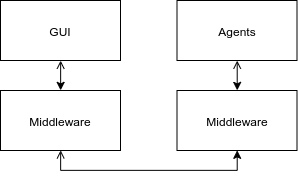
\includegraphics[width=0.5\linewidth]{images/middleware}
	\caption{Basic architecture to satisfy requirements.}
	\label{fig:middleware}
\end{figure}

\paragraph{High Level Architecture}

Due to the developer being most familiar with web technologies for creating user interfaces, a server to provide the webapp had to be included within the architecture. To avoid having to implement our agent middleware and lifecycle handling, we also opted to use JADE as mentioned in the context survey. 

JADEs agent platform (discussed in detail later) provided an API to allow other Java applications to communicate with the agents within the container. With the intention of supporting multiple simulataneous games in the future, it was decided that it made sense to have a main controlling agent as the single source of truth for each game. This main agent (later referred to as the Game agent) provides methods that allow any other agent (including the server) to subscribe to moves and chat messages.

Therefore, the server would need to maintain a mapping of users to the game agent managing their game, and would route messages received from either side accordingly. 

The final high level architecture is shown in figure \ref{fig:finalarchitecture}. To send a message from the webapp to an agent requires sending it to the server, which is able to forward the message to the corresponding game agent for a given game, which can then forward the message to the relevant pieces or just process it internally. This design was chosen as it isolated each component of the project to a single tier in the process, and could be extended to support multiple games easily. Figure \ref{fig:highlevelarchitecture} shows the same flow of data but with the technologies used at each tier, which are explained in depth later.

\begin{figure}[!ht]
	\centering
	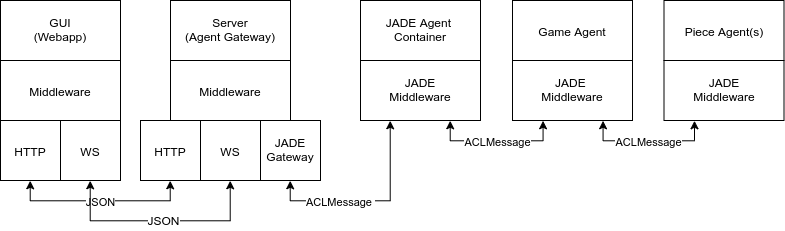
\includegraphics[width=\linewidth]{images/stacks}
	\caption{Architecture describing message passing.}
	\label{fig:finalarchitecture}
\end{figure}

\begin{figure}[!ht]
	\centering
	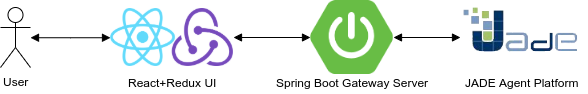
\includegraphics[width=\linewidth]{images/highlevelarchitecture}
	\caption{Technologies used at each layer.}
	\label{fig:highlevelarchitecture}
\end{figure}

\paragraph{Process}

Our player requests the webapp from the gateway server at a known address using their browser. The player provides some initial configuration for the game (who plays as white, the personalities they would like to play against, etc), and submits this information. A POST request containing the configuration is sent to the server, which creates a game agent within the agent container which then in turn creates all the piece agents needed for the game using the configuration requested by the user. 

Once all the resources are prepared, the server returns a game ID to be used by the client at a websocket endpoint which is then used for all future communication between the two components. 

When the human makes a move using the client, the move is verified locally then pushed to the server using the websocket endpoint containing the game ID, which then routes the message to the corresponding game agent, who performs the move and broadcasts that the move has occurred to the player and all the piece agents.

How agents process moves and messages is explained in more depth later, but at the highest level they are constantly in a state of discussion. One agent 'talks' at a time, either requesting the game agent to make a move, or sending a message to further the current discussion to all other piece agents in their game. These messages contain a natural language representation of the contents of the message which is forwarded to the client by the game agent. The messages have a number of fields containing information such as other moves to discuss, or justifications for choosing a certain move. 

Agents internally decide how they would like to proceed with the discussion, and each track the current conversation context to help them make this discussion. 

\subsection{Front-End}

The front end had two roles: render the game and dialogue as messages arrive, and provide a way for the user to set the initial configuration for the game. 

React \cite{reactjs} was chosen due to it being the most familiar web framework for the developer of this project. Fortunately, an open source component already existed for rendering chessboards \cite{chessboardjsx} implemented for the React framework. This library provided only the standard components of the game, and could be imported into our project and immediately provide visual elements such as the chessboard, pieces, and event handlers to allow us to perform our own processing on events such as pieces being clicked, dragged, and dropped into positions. 

We were also able to use the chess.js \cite{chessjs} library to perform tasks such as managing the local board state, and verifying moves being made by the user before sending them to the server. However, these libraries did not support features such dialogue boxes overlaid on pieces, individual nametagging of pieces, or handling of client-server communication. 

Our custom overlay for providing these extra features was implemented as individual react components. For example, a piece nametag would be considered a single component, and a piece overlay could also be a single component that would draw an array of piece nametags at the correct position on the board. Each component manages its own state and passes updates to child components (for example, the piece overlay would pass the name of the agent to each child nametag component).

The UI is composed of two main views: configuration and gameplay. 
The configuration view (Figure \ref{fig:configview}) allows the user to choose if they want to play against the agents or watch two sets of agents play against each other. By clicking on the pieces they will not be controlling, the user can also name the pieces and define their personality type. 

\begin{figure}[!h]
	\centering
	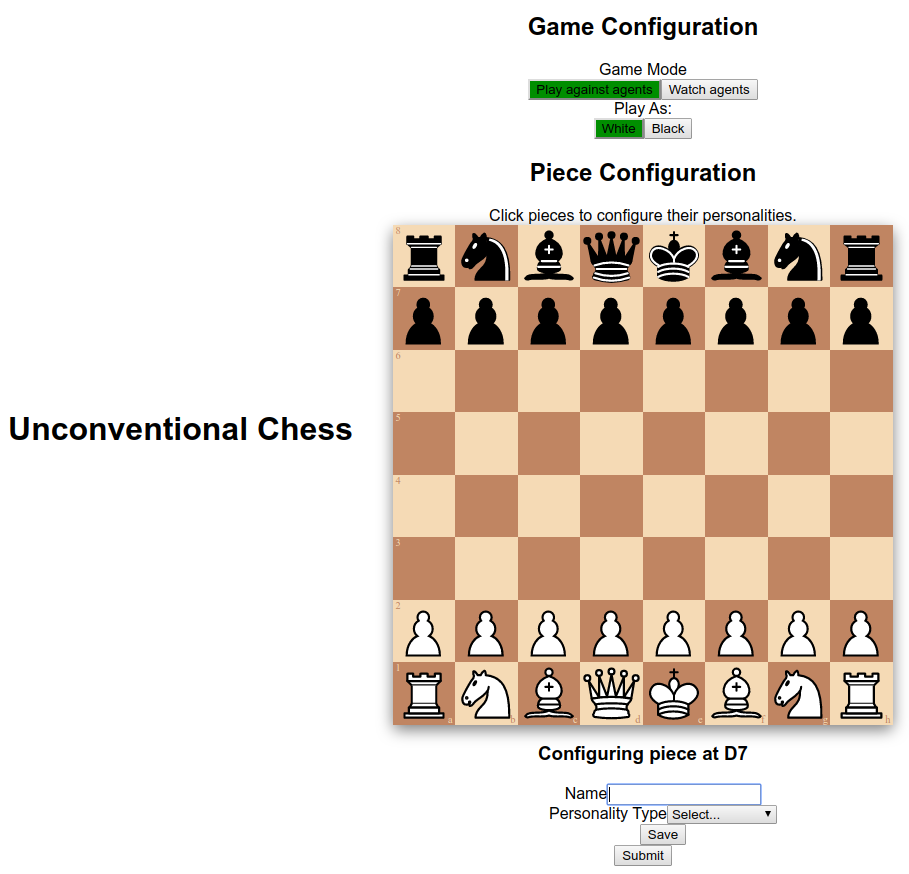
\includegraphics[width=0.9\linewidth]{images/configview}
	\caption{Configuration view.}
	\label{fig:configview}
\end{figure}

On submit, any unconfigured pieces are filled out at random from the set of available personalities and a set of names. The game configuration is then sent as a POST request to the gateway server, which verifies and creates the resources necessary for the game and returns its ID to allow the client to publish and subscribe to game events at the correct web socket endpoint.

Figure \ref{fig:gamecreation} shows the sequence diagram for how resources are created once the user submits the game configuration.

\begin{figure}[!h]
	\centering
	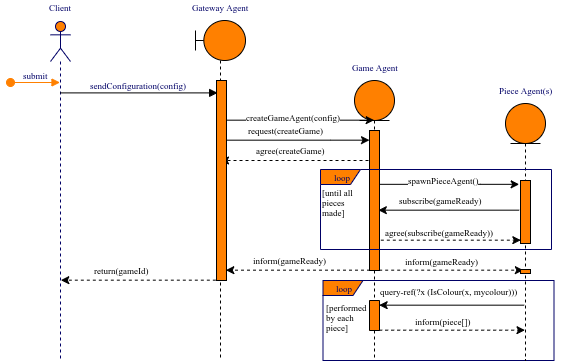
\includegraphics[width=\linewidth]{images/gamecreation}
	\caption{Game creation sequence diagram.}
	\label{fig:gamecreation}
\end{figure}

The game view (Figure \ref{fig:gameview}) also shows the game board with name tags over the corresponding pieces and any dialogue next to the speaking piece. The chat and move history is also rendered in a scrolling transcript at the bottom of the page in alternating colours for clarity. When hovering over pieces the user is able to see all currently available moves to them.  Figure \ref{fig:humanmove} shows how human moves are broadcast to all subscribers.

\begin{figure}[!h]
	\centering
	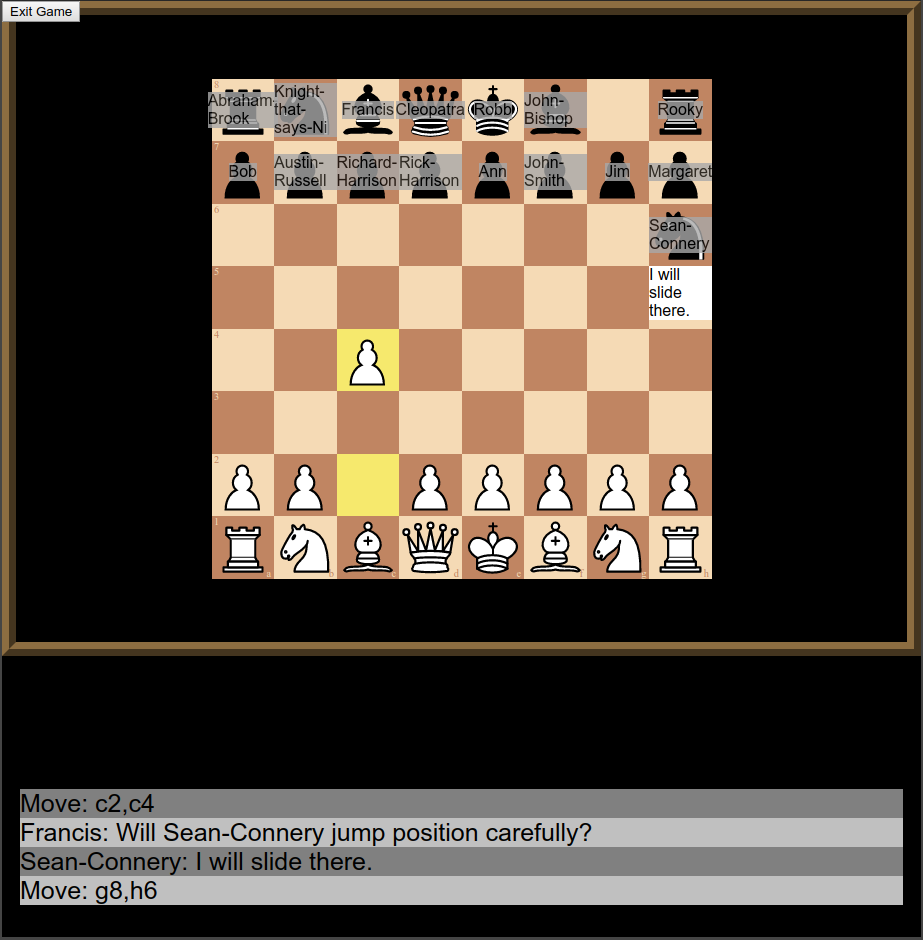
\includegraphics[width=0.8\linewidth]{images/gameview}
	\caption{Game view.}
	\label{fig:gameview}
\end{figure}

\begin{figure}[!h]
	\centering
	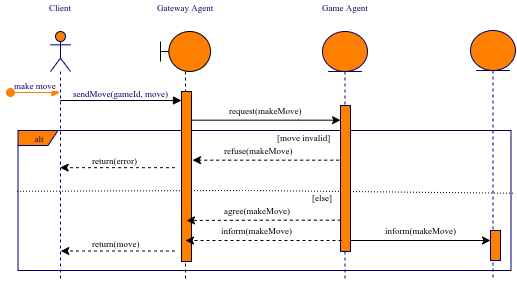
\includegraphics[width=\linewidth]{images/humanmove}
	\caption{Human move sequence diagram.}
	\label{fig:humanmove}
\end{figure}

As the project grew, Redux \cite{redux} was introduced in order to help with state management of components, as some updates would need to traverse a large number nested components. Redux provides a single global state which components 'connect' to in order to receive updates. Updates are 'dispatched' as actions, which are then passed through a pipeline of reducers which update parts of the global state depending on the action and its payload. Middleware can also be introduced to allow certain actions to create chains of updates (e.g. making an asynchronously API call, then dispatching another action when the response is received), but the reducers themselves are always pure functions. This functional approach to managing components made the project easier to test and errors easier to trace and correct. Figure \ref{fig:reducers} shows the parts of the state that are managed by each reducer.

\begin{figure}[!ht]
	\centering
	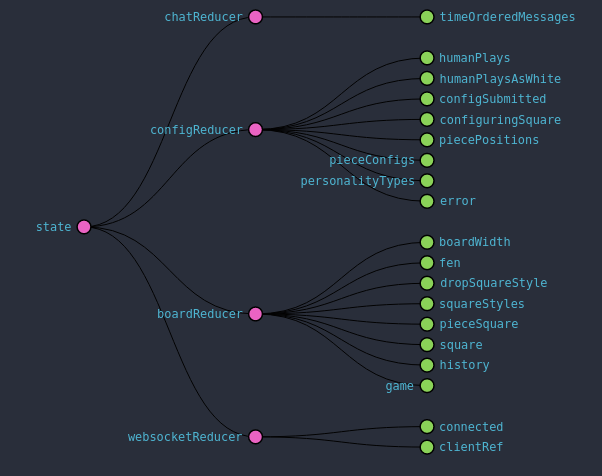
\includegraphics[width=\linewidth]{images/reducers}
	\caption{Redux reducer tree showing which parts of the state are managed by which reducers.}
	\label{fig:reducers}
\end{figure}

\subsection{Agent Gateway Server}

The gateway server has several purposes: 
\begin{itemize}
	\item{Serve the web app}
	\item{Handle game resources}
	\item{Route messages between users and relevant agents}
\end{itemize}

% TODO

JADE does have support for agents serving web resources directly, but the JadeGateway API was used instead as it was simpler to set up. The JadeGateway API effectively creates an Agent for the server, which can then send units of functionality called 'Behaviours' to be executed by the agent (e.g. sending messages to the agents within the platform). This could potentially be a bottleneck if the number of users of the server was to grow large enough due to agents being single-threaded by default, so an implementation at scale would likely need to change this interface. For the purposes of this project however, it was more than sufficient.

On start-up, the server uses the details in a configuration file to connect to the JADE platform. It also exposes a limited set of HTTP endpoints to allow the client to create games and to query available personality types. An in-memory message broker is used for handling websocket sessions once a game is set up so that clients can subscribe to chat and move messages, and send their own moves. 

In order to receive messages from agents within the container , the JadeGateway polls for incoming messages using the \lstinline{ListenForGameAgentMessages} behaviour, which is provided a message translator and a message handler for translating \lstinline{ACLMessage}s from agents to a data model the server can work with and passing the message to the correct handler. This behaviour allowed the server to utilise JADEs scheduling system which would only run the behaviour if a new message was received, instead of busy waiting for incoming messages. 

\subsection{Jade Agent Platform}

Finally, the agent platform is where all of the agents are hosted. Here we will give a rough overview of how JADE agents schedule their functions, while in section \ref{sec:agentimpl} we discuss the actual logic that drives our agents.

JADE agents are single-threaded by default, and execute behaviours according to the flow diagram shown in Figure \ref{fig:behaviour}. The basic JADE behaviour implements the methods shown in figure \ref{fig:behaviour}, but the framework also provides some helper implementations such as the \lstinline{FSABehaviour} which was used heavily during this project. 

Behaviours are scheduled such that they are executed repeatedly round-robin until either they are complete (\lstinline{done()} returns true) or \lstinline{block()} is called during the \lstinline{action()} method. The latter puts the behaviour into a waiting queue so that it is only triggered again once the agent receives a message. 

Behaviours can filter the messages that are received using the \lstinline{MessageTemplate} class, which uses pattern matching to only allow for messages containing features such as a specific performative (e.g. REQUEST, PROPOSE) or a specific conversation ID. This ensures that behaviours do not consume messages that were not intended be consumed by them. 

\begin{figure}[!ht]
	\centering
	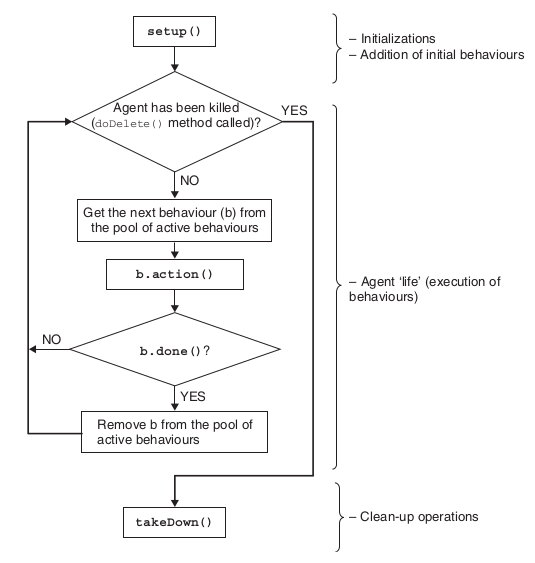
\includegraphics[width=0.8\linewidth]{images/behaviour}
	\caption{JADE Agent behaviour scheduling and life-cycle \cite{jade}.}
	\label{fig:behaviour}
\end{figure}

\section{Agent Implementation} \label{sec:agentimpl}

Our implementation involves two different types of agent: game agents and piece agents. Game agents are responsible for maintaining the state of the game and initialising the piece agents, and piece agents represent pieces on the board, each trying to achieve their own individual goals.

\subsection{Game Agent}

The game agent upon creation waits for a request to begin a chess game. It also answers any queries regarding the current status of the game and information about the pieces being represented by agents. The FIPA standard protocols for agent interaction \cite{fipaprotocols} were followed so that the game agent could provide a consistent API for any implementation of piece agents. For example, the request interaction is used for triggering moves as shown in figure \ref{fig:humanmove}. 

Requests for information are semantic logic expressions with variables which the game agent then populates in its reply. For example, agents wishing to receive updates whenever a new move is made will send a message with a SUBSCRIBE performative and the expression:

\begin{equation} \label{eq:movesubscribe}
	(\;iota\; ?Move\; ("Move Made"\; ?Move))	
\end{equation}

This will then be replied to every time a new move occurs with the variables given values, for example when a piece moves from B8 to C6:

\begin{multline} \label{eq:movesubscriberesponse}
	((=\; (iota\; ?Move\; ("Move Made"\; ?Move))\;  \\
	(Move\; :Source\; (Position\; :Coordinates\; B8)\; \\
	:Target\; (Position\; :Coordinates\; C6))))
\end{multline}

Once the game has started, the game agent adheres to the FSA shown in figure \ref{fig:gameagentfsa}. 

\begin{figure}[!ht]
	\centering
	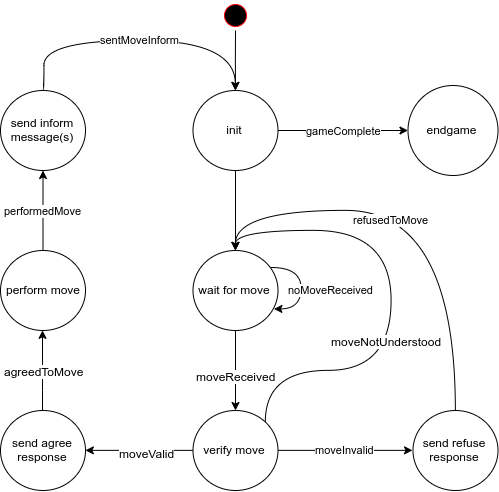
\includegraphics[width=0.8\linewidth]{images/gameagentfsa}
	\caption{Game Agent game handling FSA.}
	\label{fig:gameagentfsa}
\end{figure}

The actual chess logic is managed by a third party library \cite{chesslib}. While this saved a lot of time by providing a way of quickly validating moves, generating valid moves, and tracking the board state, it suffered from the same problem as the chessboard component used by the front-end: it did not provide a way to differentiate between each piece of the same type. This resulted in a wrapper class being implemented which would maintain the mapping between the set of our custom piece representation and the third party board pieces. In hindsight it was clear that it would have been simpler to have implemented the chess logic ourselves, but the wrapper solution was sufficient.

\subsection{Piece Agent}

The piece agent implementation is the focus of this project. They are initialised with their piece type, colour, personality type, and starting position on the board. They are notified by the game agent once the game is ready and whenever a move is made successfully either by the human or another agent. 

\subsubsection{Game State}

The GameState class wraps our chessboard wrapper to provide another layer of abstraction in order for the state of the board to be an immutable object. This was done to avoid complicated undo logic when agents wanted to 'test' moves and evaluate the board after a move is made. Instead, when the \lstinline{applyMove(PieceMove move)} function is called, a copy of the board is made. This involved copying the set of alive and captured pieces, as well as updating the piece objects themselves if any changed position. 

In order to reduce the amount of objects being created and destroyed by this process, piece instances would only be copied if they had changed state in some way (captured/changed position). 

\subsubsection{Personalities and Reasoning}

Agent personalities were designed based on the goal-based trait/value model defined by \cite{hetrogenousagents}. Figure \ref{fig:personalityuml} shows the UML class diagram for our implementation. The personality is initialised with a set of traits (e.g. shy, aggressive) which each have a set of values. Values define what the agent will interpret as good and bad moves based on some criteria (avoid other pieces, maxmise captures). The value class is abstract and is extended by implementations that when given a witnessing piece, the current game state, and a move, are able to produce a response to that move.

\begin{figure}[]
	\centering
	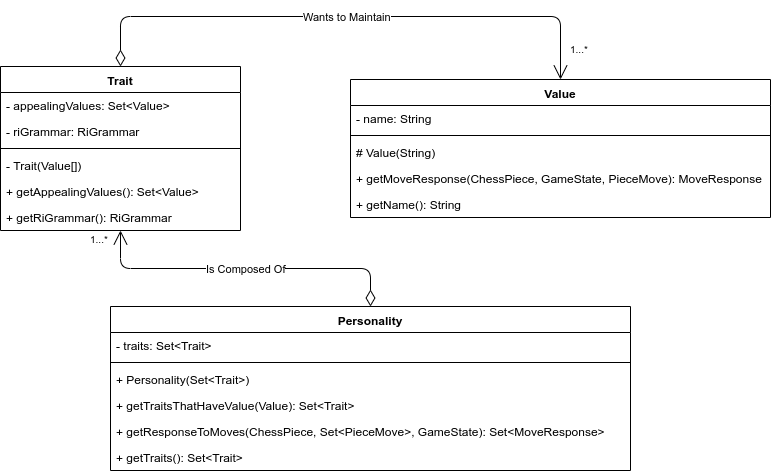
\includegraphics[width=0.8\linewidth]{images/personality}
	\caption{UML Diagram of Agent Personalities.}
	\label{fig:personalityuml}
\end{figure}

This implementation allows different traits to share goals. The move most preferred by an agent is the one that appeals to the most of it values, and so consensus can be reached by finding the move that appeals to the most pieces, even if they have different values.

\subsubsection{Single Thread of Conversation Protocol}

In order to make the conversation between agents seem natural and remain easy to follow, a protocol had to be established to ensure that one agent would speak at a time. The project was initially constructed with conversation flow dictated strictly by a finite state machine. This solution was incredibly restrictive as it required providing a transition path for any conversation path that we wanted to support. After reviewing the work by \cite{tartan} and finding that this strict FSA approach was inherently detrimental to producing natural conversation flows, the original design was thrown out and replaced with the simpler and far more flexible model shown in Figure \ref{fig:conversationfsa}.

\begin{figure}[]
	\centering
	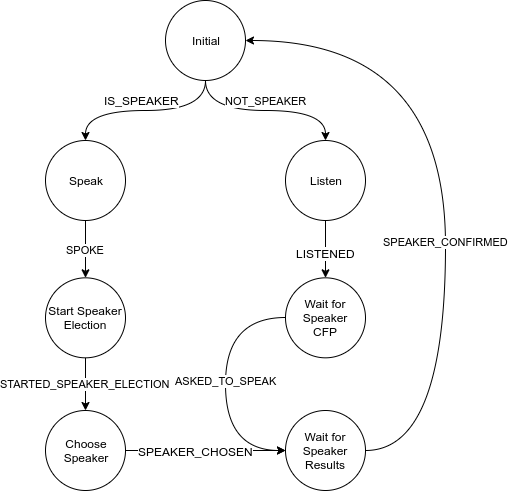
\includegraphics[width=0.8\linewidth]{images/conversationfsa}
	\caption{Conversation protocol FSA}
	\label{fig:conversationfsa}
\end{figure}

The conversation FSA designed by \cite{tartan} was for a human-agent chatbot, and so was adapted to include a token-passing protocol to determine which agent would speak next. One of the benefits of this design is that it allowed for the agents to chat throughout the game, not just during their turn. This meant that the agents could provide ambient conversations and respond to events like the previously made move while the human player chose their next move.

At the start of each turn (i.e. when a new move is received or the very first turn of the game), each agent returns to the initial state to ensure that they are all synchronised. The king is assumed first to speak. The other pieces listen for any messages from the speaker and the speaker chooses what to say. Once sent, the speaker begins the new speaker election by sending a call for proposal (CFP) message to all alive pieces (and themselves), and waits until every pieces has submitted a proposal to be the next speaker. Finally the speaker chooses from the set of proposals, sends a rejection to all but the chosen speaker, and then the cycle begins anew.

If the agent chooses to make a move while they are speaker, they transition into the corresponding state as shown in figure \ref{fig:conversationfsa}. They remain here until they receive either a refuse or agree response from the game agent and then return to the normal conversation cycle. 

The requirement that all agents reset to the initial state at the start of each turn was necessary to avoid race conditions during the speaker election. For example, if a move was received that resulted in one of the agents being captured, that agent would immediately remove themselves from the game. However, if that agent was the speaker during an election, then all other agents would be stuck waiting for the next speaker to be chosen. Whilst other solutions would allow for the conversation flow to continue, it was deemed much simpler to reset the conversation FSA during each turn.

As a side effect of this decision, messages such as the speaker election CFP could be waiting in an agents message queue if they reset before receiving it. To avoid this resulting in a loss of synchronisation between agents, a new conversation ID is assigned during each cycle of the FSM which is composed of the turn ID (i.e. how many moves have been made so far) and the round ID (how many cycles of the conversation FSA have occurred this turn). The conversation ID is used to filter incoming messages to ensure that irrelevant messages are ignored. Unfortunately this could result in a build-up of expired messages over time, but given most chess games are around 80 moves \cite{chessdata} and roughly 5 messages per move would be lost in the queue, the leak would not be substantial. Especially when it was considered that the messages would be garbage collected once the agent representing the piece was removed from play.

The turn and speaker rotation counters is provided by the ConversationContext class, along with the current speaker agents AID (Agent Identifier) and the conversation planner. 

\subsubsection{Conversation Planner and Argumentation}

Each agent maintains a conversation planner which tracks what moves have been discussed so far, and produces a response for this agent once it has its turn to speak. Figure \ref{fig:movediscussion} shows the classes used to maintain this information.

\begin{figure}[]
	\centering
	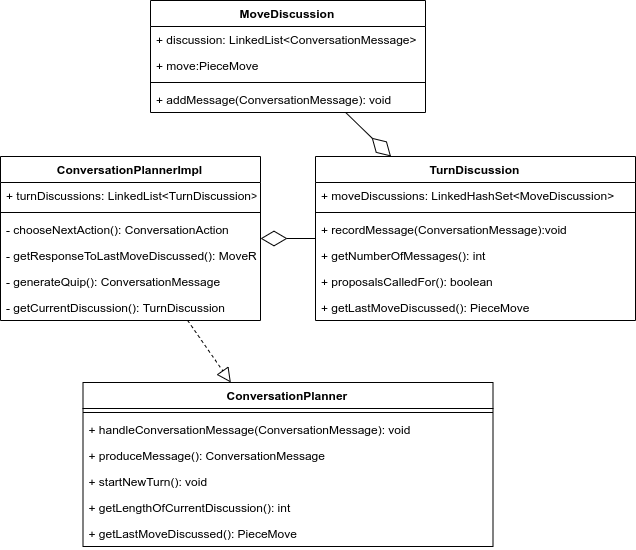
\includegraphics[width=0.8\linewidth]{images/movediscussion}
	\caption{Move Discussion Class Diagram}
	\label{fig:movediscussion}
\end{figure}

Whenever an agent enters the speaker state shown in figure \ref{fig:conversationfsa}, they call the \lstinline{produceMessage()} function to choose their next action. If this action involves making a move, they'll queue a behaviour to send the move to the game agent. Regardless, they send their chosen conversation message to all the other agents (including themselves).

Listener agents receive the conversation message and record it by calling the \lstinline{handleConversationMessage(ConversationMessage)} method. The conversation planner delegates storing the message to the current turn discussion (the head in the list of discussions). The turn discussion will fetch the move discussion for the move in the given conversation message or create a new one if one doesn't already exist and add the message to the relevant move discussion. Once the message is added to the move discussion, the discussion is removed and re-added to the set of move discussions in order to move it back to the top of the converstation 'stack' (since insertion order is maintained by Java's LinkedHashSet implementation). 

By maintaining the order that moves have been discussed, agents are able to create arguments that better resemble human conversations by referring to previous discussions. \cite{tartan} uses a similiar technique to allow their chatbot to regress to previous topics of discussion once the user gives some kind of terminating statement to the current topic of conversation. 

A move discussion with a null move is used to represent a request for move proposals, which is sent either to start up the argumentation process or when an agent is not satisfied with the move currently being discussed but is does not feel strongly about any moves themselves.

The output of \lstinline{chooseNextAction()} in the \lstinline{ConversationPlannerImpl} is the next conversation action to be taken. These actions are essentially transitions which control the flow of the conversation and are based off the interruption FSMs in Tartan \cite{tartan}. Table \ref{tbl:conversationaction} lists examples of the conversation actions possible. The actions prefixed with wildcards can be used in conjuction with other actions. For example, an agent can voice opinion with justification, or voice their dislike and propose an alternative. 

\begin{table} 
\centering
\caption{Conversation actions with verbalised examples.} 
\label{tbl:conversationaction}
\begin{tabular}{ r|l } 
	Conversation Action & Example \\
 \hline
	Acknowledge & "Ok." \\ 
	Ask for Proposals & "What should we do next?" \\ 
	Perform Move & "Going to move to A5." \\ 
	Propose Move & "What about B4 to B3?" \\ 
	Revisit Move & "Let's go back to talking about the move to G7." \\ 
	Voice Opinion & "I like that idea!" \\ 
	* Propose Alternative & "but we could also move to G3." \\ 
	* Propose Compromise & "moving to G3 would do that too"  \\ 
	* with Justification & "because it would capture an enemy."  \\ 
	Quip & "I'm a bit scared."  \\ 
 \hline
\end{tabular}
\end{table}

Each of these actions are implemented as classes that extend the ConversationAction class shown in Figure \ref{fig:conversationmessage}, and once performed they return a ConversationMessage instance with all the information needed for other agents to update their own understanding of the conversation context. The actions can also extend each other if their affect on the conversation flow is the same but the natural language representation needs to differ (for example, revisiting a previously discussed move and proposing a new move both begin a new move discussion but would be expressed differently in english).

\begin{figure}[]
	\centering
	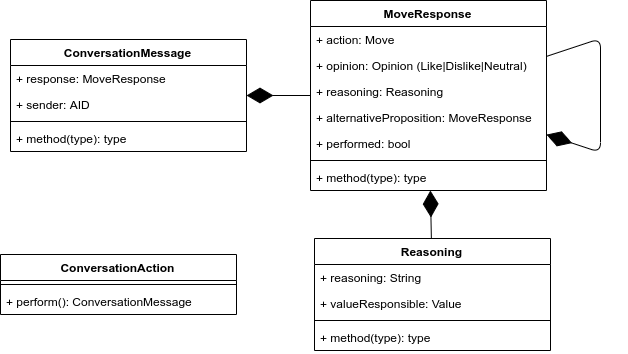
\includegraphics[width=0.8\linewidth]{images/conversationmessage}
	\caption{Conversation Message Class Diagram}
	\label{fig:conversationmessage}
\end{figure}

Conversation messages contain the name of the piece that sent it, the natural language representation of what the agent wanted to communicate, and a move response. The mapping between each field and agent intentions are described in table \ref{tbl:conversationmessagemeaning}. The alternative proposition field starts a new move discussion if present and the same logic is applied recursively as though it was the the move response in the original conversation message.

This information is enough to allow agents to determine how other agents feel about the move being discussed and make decisions about what conversation actions would logically follow, but the contents of the statement in the ConversationMessage are completely flexible.

\begin{table} 
\centering
\caption{Conversation message fields and the agent intention.} 
\label{tbl:conversationmessagemeaning}
\begin{tabular}{ l|l|l } 
	Field & Predicate & Agent Intention \\
 \hline
	response & == null & Requested proposals \\ 
	response.opinion & != null & Voiced opinion \\ 
	response.reasoning & != null & Gave justification \\ 
	response.alternativeProposition & != null & Proposed alternative \\ 
	response.performed & == true & Performed move \\ 
 \hline
\end{tabular}
\end{table}

The next conversation action is chosen by building up the set of responses that would make sense given the discussion so far and then selecting one from the set randomly. Most responses are equally likely, but some are given lower likelihoods of occurring (such as performing a move) in order to extend conversation and encourage discussion rather than agents just repeatedly proposing their own preferred moves.

Choosing responses that 'made sense' involved checking the current discussion context and determining the following:
\begin{itemize}
	\item Is this the first message this turn?
	\item Did the previous message ask for proposals?
	\item Have moves been discussed already?
	\item What is this agents opinion of the move currently being discussed?
	\item Does a move exist that I can perform?
\end{itemize}

In order to create the illusion that pieces are moving themselves, only the speaker can perform a move and that move has to involve the same piece. This choice will likely result in less strategic moves being made (for example, a piece will not want to put itself at risk, even if it means saving a more important piece), but makes for a more entertaining narrative.

The reasoning field in move responses are populated by the Value of an agent assessing a given move. This gives a natural language explanation for the value of the opinion field in the move response, and the value that was used to compute it. This allows other agents to apply the same value to all other moves (even if they do not have that value themselves) and provide a compromise that also appeals to their own values. 

This argumentation feature could be improved by expressing the value as a predicate that other agents could unpack instead of being tied to the Value classes in our chess agent library. 

The conversation planner was extended to support reactions as well as discussion actions. This allowed agents to respond both to their moves and to the users moves to try and improve immersion.  A hard limit was placed on the number of reactions to the enemies moves on the start of a turn to avoid discussion being delayed by an unrealistic number of reactions from different pieces. The type of reactions that could be performed managed by checking previous conversation frames and the game state resulting from the move performed.

\begin{table} 
\centering
\caption{Reactions with verbalised examples.} 
\label{tbl:reactions}
	\begin{tabular}{ p{0.4\linewidth}|p{0.6\linewidth} }
	Reaction & Example \\
 \hline
	Compliment Enemy Move & "Oh no, that was a pretty good move by their Knight" \\ 
	React to Enemy Piece Captured & "Haha! We have your Bishop!" \\ 
	React to Friendly Piece Escaping & "Good, John is safe now!" \\ 
	React to Last Move Discussed Being Performed & "I'm glad you agreed to that move!" \\ 
	React to Undiscussed Move Being Performed & "...Maybe ask next time before moving, Kate." \\ 
 \hline
\end{tabular}
\end{table}

These reactions required slightly more complex checks to the discussion actions as they were dependant on very specific changes in the game occurring to make sense.

\subsubsection{Natural Language Generation}

The natural language generation was a crucial part of this project, as it had to tie together all other features correctly in order to make their effect visible to the user. The phrases spoke by pieces had to:
\begin{itemize}
	\item correlate to the opinion of the pieces and the moves being discussed
	\item vary enough to not appear scripted
	\item make grammatical sense when combined 
	\item make sense with respect to previous statements by other agents and themselves
	\item be consistent with the personalities of the individual pieces
\end{itemize}

As mentioned in the context survey, the development of the natural language generation aspect of this project was greatly slowed down by starting off with likely the wrong technology for the problem. SimpleNLG appeared to be useful given a better understanding of linguistics, and so a lot of time was spent understanding the technical terms of this field. However, the tool seemed better suited to tasks like report generation than conversation, and so with assistance from the project supervisors, the RiTa libary was adopted instead.

RiTa provides a wealth of features for natural language processing and generation, but the determinstic grammar was especially useful for this project. Phrases are constructed from non-deterministic BNF grammars and a datasoure for filling in variables such as agent names or move coordinates. A default grammar is provided, but by implenenting variations of the default grammar for each trait, agents will express themselves based on the traits of their personality. A root tag is provided for each class that extends ConversationAction. For example, the ProposeMoveWithJustification conversation action used a grammar similar to example shown in figure \ref{fig:bnf}. Multiple values can be provided for each tag by adding them to the array of values for that key, and the probability of each value being chosen can also be defined using square brackets within the string to multiply the probability of it occurring (i.e. [2] will make the value be chosen twice as often as any of the other values in the array).

\begin{figure}
\begin{lstlisting}[breaklines=true, stringstyle=\color{mauve}]
"<ProposeMoveWithJustification>" : 
	["<ProposeMove> <Justification>"]

"<ProposeMove>" : 
	["`getMovingPiece()` should move to `getMoveTarget()`"]

"<Justification>" : 
	["because that move `getJustification()`"]
\end{lstlisting}
\caption{Example of BNF grammar being used for NLG.}
\label{fig:bnf}
\end{figure}

Each value also uses a BNF grammar to produce the justification in natural language, but these are implemented within the values themselves rather than as separate schemes.

The strings between backticks within the grammars are slots that are express the name of a field or a function call that will provide the value for the slot in the GrammarVariableProvider. This is an object populated with things like the name of the agent being asked to move and the coordinates being moved to.

\section{Evaluation}

The success of the resulting software was ascertained by analysis its performance ourselves and by gathering user feedback. Issues raised by these assessments were later addressed to produce the final artefact that was included with this submission.

\subsection{Strategic Analysis} \label{ss:sa}

In order to test the strategic performance of the implementation, the Stockfish engine \cite{stockfish} was used to score the move chosen at each turn by the agents. This was repeated over the course of five games to account for the randomness used by agents during the choice of action. Different configurations of personalities for pieces were used for each game.

Stockfish is one implementation of the universal chess interface and one of the best chess AIs in the world. It uses a complex set of rules to score board positions, which can be used to identify the next best move to make. Centipawns are the unit used for the score produced, which represent one hundredth the value of a pawn (1 point). The king is essentially of infinite value, and so for our data we translate mating moves to centipawns by assigning these moves an arbitrarily large number, as recommended in the \lstinline{python-chess} documentation \cite{pythonchess}. 

The moves were tracked by adding a logger to the game agent which would record the current position in the standard Forsyth-Edwards Notation (FEN), and the source and target of the move being made. Both teams were represented by agents and the conversation delay set to a much lower number to increase the rate of discussion. The comma separated value dataset produced was then parsed by a python script. For each position recorded, all legal moves were considered by Stockfish with a limit on the computation time of one hundred milliseconds per move. This produced a score for all legal moves at each position including the chosen move.

In figure \ref{fig:scoreovergame}, the difference between the maximum possible scoring move and the score given to the chosen move is plotted for each turn and for each game. Points closer to the x-axis represent moves that could be considered good. Due to mating moves being of very high value, whenever these moves were not chosen the difference is much higher, and so figure \ref{fig:scoreovergamefiltered} was also plotted with these moves filtered to give a better visualisation of the agents performance over time.

\begin{figure}[]
	\centering
	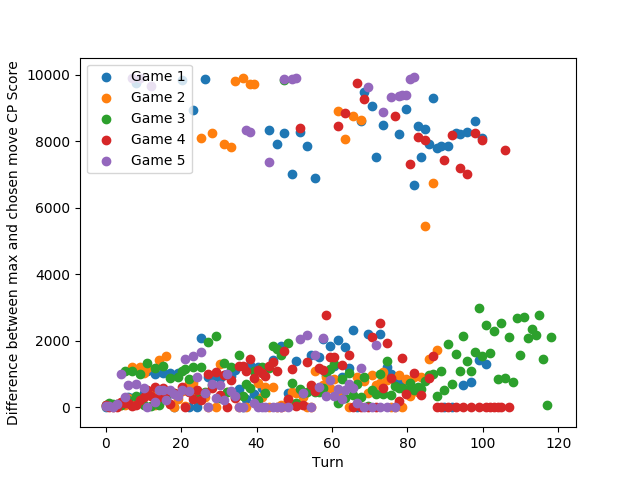
\includegraphics[width=0.8\linewidth]{images/score_over_game}
	\caption{Differences between best move and chosen move score over the course of five games}
	\label{fig:scoreovergame}
\end{figure}

\begin{figure}[]
	\centering
	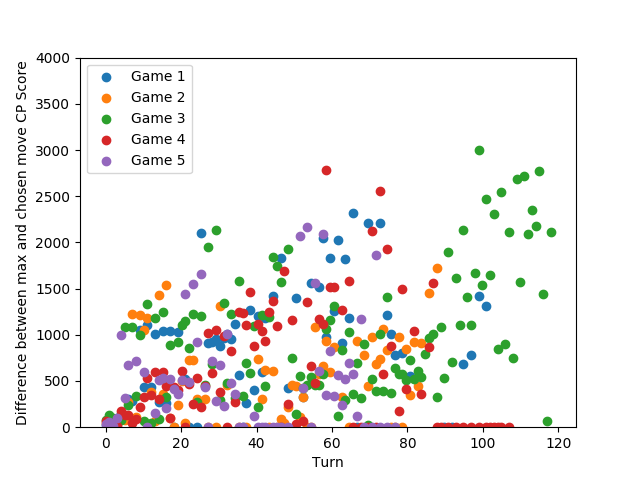
\includegraphics[width=0.8\linewidth]{images/score_over_game_filtered}
	\caption{Figure \ref{fig:scoreovergame} with differences over 4000 removed}
	\label{fig:scoreovergamefiltered}
\end{figure}

Figure \ref{fig:scoreovergame} shows that often the mating moves were not taken, and this was likely due to the fact that no value was implemented that would trigger a LIKE reaction if the threatened piece was the enemy king specifically. This highlighted the need for piece value to also be accounted for when choosing moves if the agents were to have any strategic advantage, but this would likely also require introduced a numerical scoring of moves by agents instead of the three value (LIKE, NEUTRAL, DISLIKE) approach taken.

Interestingly, certain games seemed to have produced better moves which could suggest that either 
\begin{enumerate}
	\item Certain personalities were more effective at choosing good moves and these personalities were more represented for that game. For example, the aggressive personality type would maximise captures, reducing the number of opponents, which would be evaluated as high scoring moves due to capturing pieces being worth a large number of centipawns.

	\item Certain combinations of personalities were more effective when combined in a given ratio. For example, having a balance of aggressive and defensive personalities would result in moves that would capture pieces whilst maintaining the least number of threatened friendly pieces.
\end{enumerate}

\begin{figure}[]
	\centering
	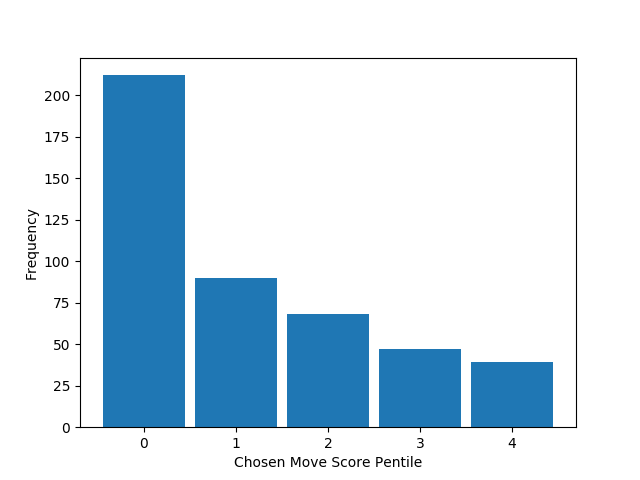
\includegraphics[width=0.8\linewidth ]{images/frequency}
	\caption{Frequency of chosen move being in each score pentile}
	\label{fig:frequency}
\end{figure}

To give a general overview of how well the agents performed, the scores from all moves from all games played were all collected. For each position, all the legal moves were separated into equally sized pentiles by score. The zeroth pentile contained the lowest scoring moves and the fourth the highest scoring moves. For each move, we determined which pentile the move belonged to, then plotted the frequency of the moves occurring in each percentile, and the result is shown in figure \ref{fig:frequency}.

This clearly shows that most moves taken were the least advantageous strategically, though there were still occurrences of good moves. However, if we assume that randomly chosen moves would produce an equal distribution in each percentile (though this is unlikely), then of the 496 moves considered 90 would have been in the highest percentile. Compared to our results where we have nearly half of that value, there is clearly a need to implement more strategic move evaluations if the game is to be more challenging.

\subsection{Conversation Analysis}

The fluidity of the conversations produced was challenged throughout development. Due to the complexity of natural conversation, testing for messages that made sense in series was difficult without simply rewriting the same logic being used to choose actions in the tests, and so most of the evaluation of this feature was done by manual inspection.

During the agent-vs-agent experiments discussed in section \ref{ss:sa}, conversation dialogue was not disabled, which meant that at the end of each experiment a transcript was available. Due to the rate of messages coming in, it was impossible to read and follow the discussion in real time.  The level of noise when both sides were creating dialogue made it difficult to follow even with the rate of conversation greatly reduced which made it clear that this game mode would likely be improved by only showing the dialogue from one side.

The transcripts showed more variety was likely needed in the speech corpus, as repetition was quite easy to spot when the number of messages were this large. For normal gameplay, this would be less of an issue, but it did not seem like there was enough variety in speech to make a full game entertaining. Unfortunately, this does identify a drawback with our approach: creating believable dialogue required manually curating the dataset which could take a large amount of time. However, the context free grammar approach meant that poorly formed sentences could be easily fixed as the pattern used to create the sentence could be traced.

Determining if the discussions complimented gameplay required simply playing the game and allowing the pieces to talk for a while between turns. During development, this approach identified problems such as too many reactions in a row occuring, or moves being performed too early on in the dicussion and cutting it short.

\subsection{User Feedback}

Since the goal of this project was to essentially create a video game, it made sense to take inspiration from industry standard Game Engagement Questionnaire \cite{geq}. This questionnaire is often used during user feedback sessions to measure the absorption, flow, presence, and immersion a game provides. It is comprised of a series of statements such as "I lose track of time" and "Things seem to happen automatically". For each statement, the user completes a Likert scale ranking of how much they agree with it.

Presence is a measure of how much the player feels part of the game. Due to the players pieces being fairly static, the game was not expected to score well in this area. Similarly, flow is a measure of much the players movement and interactions with entities within the game feel natural. Again, chess does not cater to this metric well due to essentially one method of interaction: moving a piece. 

On the other hand, absorption and immersion try to capture how much players become unaware of their actual surroundings due to a game. If the dialogue and conversation flow is believable enough, it is possible that the game could score fairly high in this regard.

Due to the short length of time that user feedback sessions could take, some questions were removed from the questionnaire to allow for other types of questions to be asked specific to this project.

% TODO refer to context survey content
With all the above considered, we created the questionnaire as described by table \ref{tbl:questions}. 11 participants from the school of computer science helped by taking part in the feedback exercise. The exercise involved showing the participant three short videos of gameplay in different situations to try highlight features such as reactions and piece argumentation. They were then given a few minutes to play themselves. Finally, the user was asked to complete our questionnaire. Some wanted to continue playing after this stage to try and explore the range of conversation possible, and comments made from this period were noted for future improvement.

\begin{table}[!ht]
	\caption{Questionnaire content with the question statement, the answer format (Likert meaning 5 point scale composed of strongly disagree, disagree, neutral, agree, strongly agree), and the justification for including the question in the questionnaire.} 
\label{tbl:questions}
	\makebox[\textwidth]{\resizebox{1.3\linewidth}{!}{\def\arraystretch{1.5}%
	\begin{tabular}{ r|c|p{0.7\linewidth} }
		\textbf{Statement} & \textbf{Format} & \textbf{Purpose} \\
 \hline
		I have played chess before & Yes /No & May highlight the need for more visual cues to explain rules, or possible help identify if the game could be used to educate new players how to think tactically.  \\ 
 \hline
		I am good at chess & Likert & Players who are already very familiar with chess might have different experiences to those who rarely play, and this may be observable from what we collect. \\
 \hline
		I lose track of time & Likert & Measuring presence, do players find themselves 'hooked'. \\
 \hline
		I feel different & Likert & Measuring absorption, are they emotionally affected by the anthropomorphic pieces.  \\
\hline
		The game feels real & Likert & Measuring flow, do players really feel like they are against an army of other pieces. \\
\hline
		If someone talks to me, I don't hear them & Likert & Measuring flow, do players get involved enough to not be distracted by outside influences.  \\
\hline
		I get wound up & Likert & Measuring flow. Does the game frustrate the player, are they invested in it?  \\
\hline
		I lose track of where I am & Likert & Measuring presence. Is the player focused on the game? \\
\hline
		I play without thinking about how to play & Likert & Measuring flow. The difference between experienced and non-experienced chess players may be reflected by this question also. \\
\hline
		Playing makes me feel calm & Likert & Measuring presence. Do players enjoy their time. \\
\hline
		I really get into the game & Likert & Measuring immersion. Do players really start considering the dialogue of the other pieces while playing.  \\
\hline
		I feel like I just can't stop playing & Likert & Measuring flow. Does the piece interaction interest players enough to make them keep playing. \\
\hline
		The pieces spoke with linguistic accuracy & Likert & Did the conversation make sense and not contain any gramamtical errors. \\
\hline
		The pieces had convincing, natural interactions & Likert & Did the flow of conversation feel natural and emulate human discussion.  \\
\hline
		The reactions of pieces affected me & Likert & Did the dialogue create an emotional response, for example when a piece cried out at the loss of its friend did the player feel guilt. \\
\hline
		The pieces convey personality & Likert & Is the player able to identify personality traits for each piece consistently. \\
\hline
		The pieces provide emotional information through tone & Likert & Can the player tell if a piece has expressed anger, sadness, happiness through choice of words. \\
\hline
		The dialogue made the game more fun and interesting & Likert & Did the dialogue add to the experience of playing chess, or just distract or detract from it. \\
\hline
		Comments & Free text & Allow participants to highlight anything that was especially good or bad about the game. \\
 \hline
\end{tabular}}}
\end{table}

The results from the questionnaire were taken from paper to csv, and the frequency of each answer for each question plotted. Figures \ref{fig:qfirst} to \ref{fig:qlast} show the results for each question in order.

\begin{figure}[!ht]
\centering
\begin{subfigure}{.5\textwidth}
    \centering
    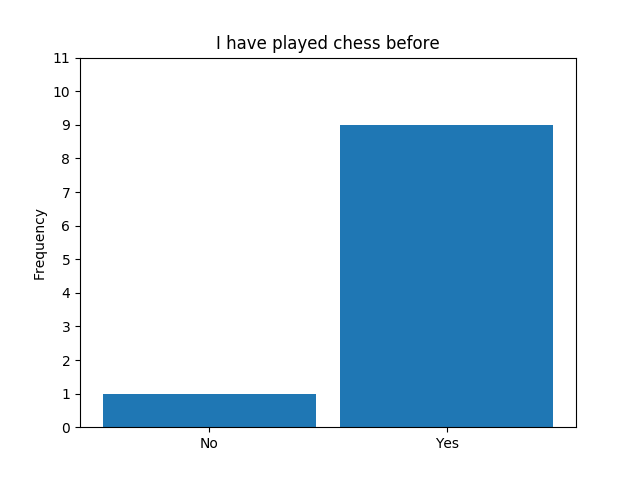
\includegraphics[width=\textwidth]{images/questions/0}
\end{subfigure}%
\begin{subfigure}{.5\textwidth}
    \centering
    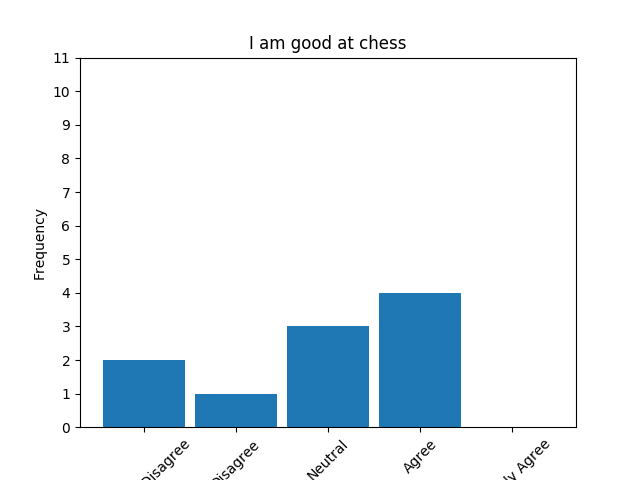
\includegraphics[width=\textwidth]{images/questions/1}
\end{subfigure}
\begin{subfigure}{.5\textwidth}
    \centering
    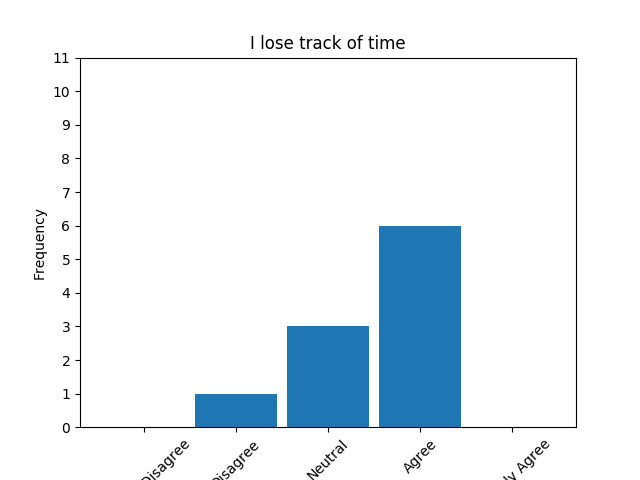
\includegraphics[width=\textwidth]{images/questions/2}
\end{subfigure}%
\begin{subfigure}{.5\textwidth}
    \centering
    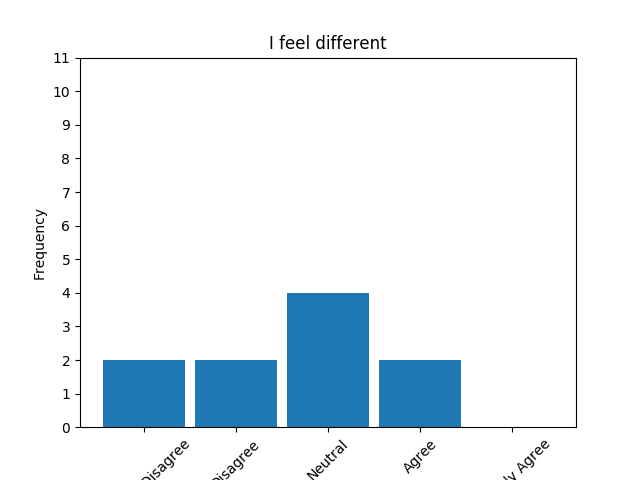
\includegraphics[width=\textwidth]{images/questions/3}
\end{subfigure}
\begin{subfigure}{.5\textwidth}
    \centering
    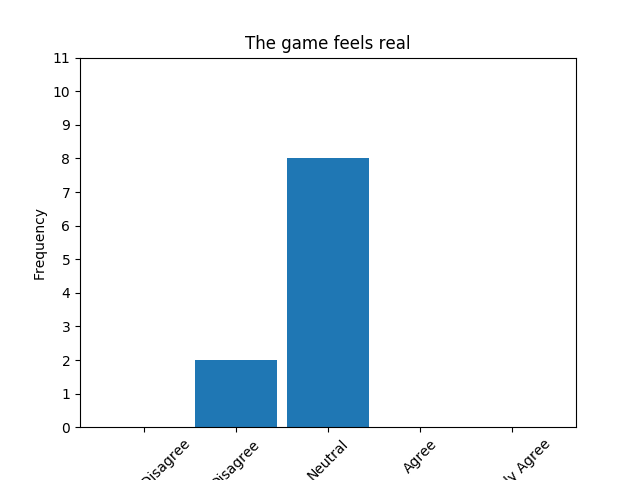
\includegraphics[width=\textwidth]{images/questions/4}
\end{subfigure}%
\begin{subfigure}{.5\textwidth}
    \centering
    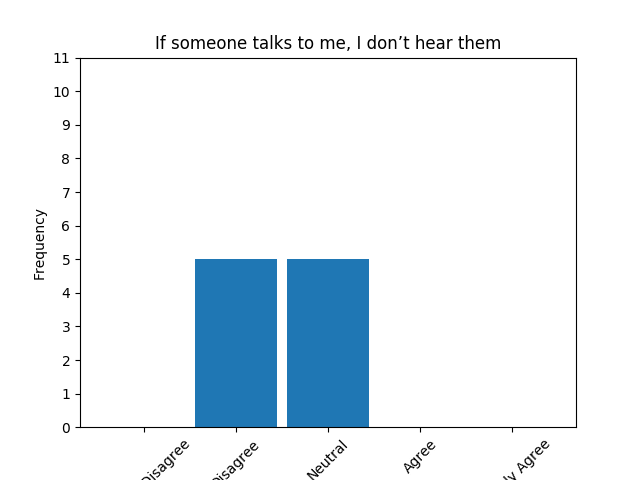
\includegraphics[width=\textwidth]{images/questions/5}
\end{subfigure}
\begin{subfigure}{.5\textwidth}
    \centering
    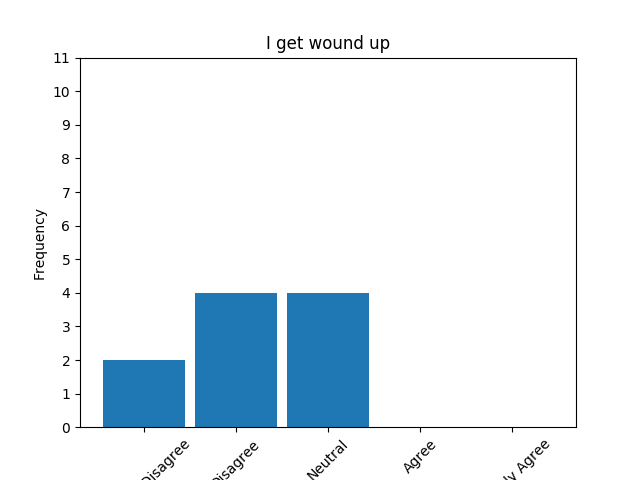
\includegraphics[width=\textwidth]{images/questions/6}
\end{subfigure}%
\begin{subfigure}{.5\textwidth}
    \centering
    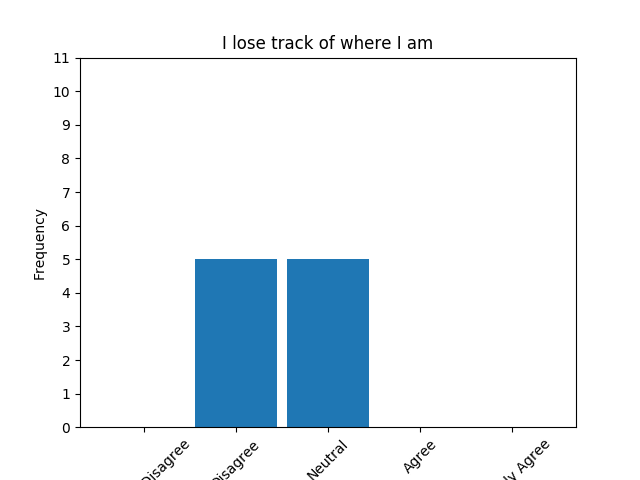
\includegraphics[width=\textwidth]{images/questions/7}
\end{subfigure}
\caption[short]{Questions 1-8 in Questionnaire}\label{fig:qfirst}
\end{figure}

\begin{figure}[!ht]
\centering
\begin{subfigure}{.5\textwidth}
    \centering
    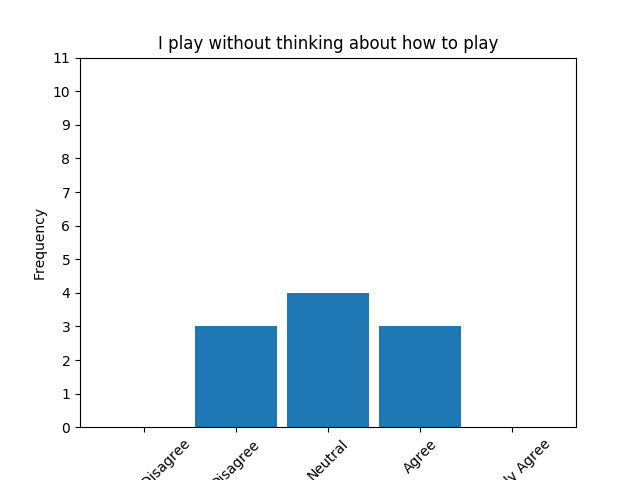
\includegraphics[width=\textwidth]{images/questions/8}
\end{subfigure}%
\begin{subfigure}{.5\textwidth}
    \centering
    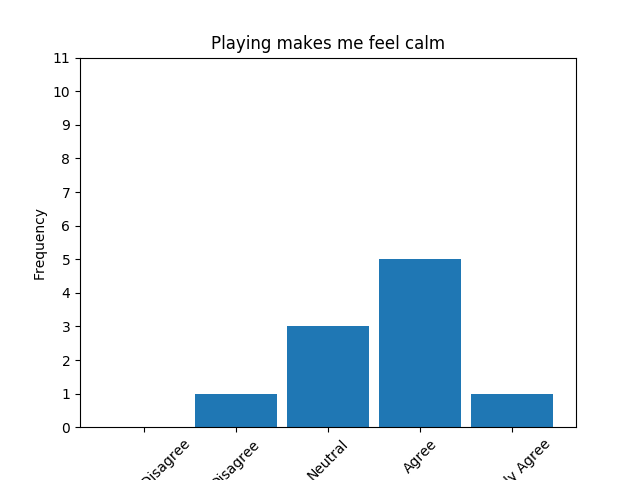
\includegraphics[width=\textwidth]{images/questions/9}
\end{subfigure}
\begin{subfigure}{.5\textwidth}
    \centering
    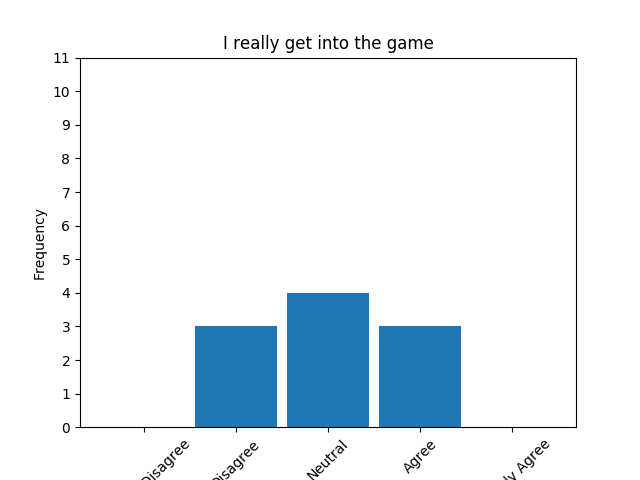
\includegraphics[width=\textwidth]{images/questions/10}
\end{subfigure}%
\begin{subfigure}{.5\textwidth}
    \centering
    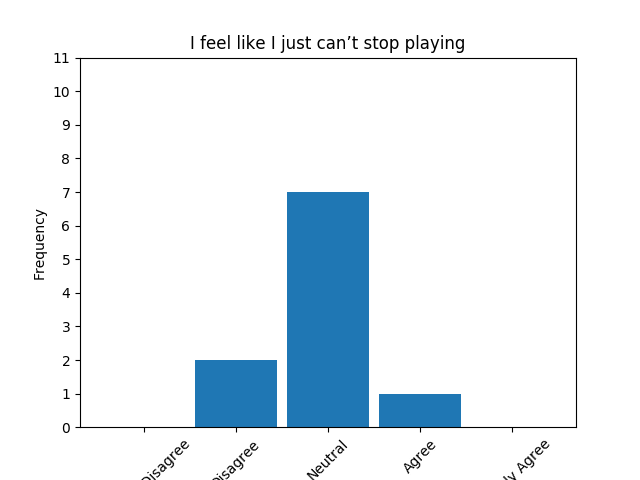
\includegraphics[width=\textwidth]{images/questions/11}
\end{subfigure}
\begin{subfigure}{.5\textwidth}
    \centering
    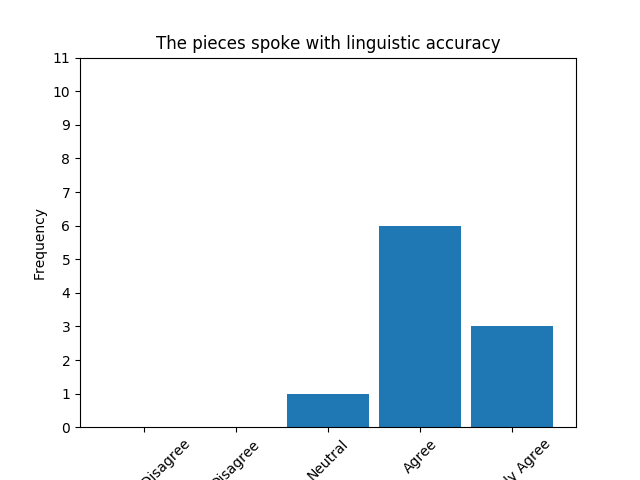
\includegraphics[width=\textwidth]{images/questions/12}
\end{subfigure}%
\begin{subfigure}{.5\textwidth}
    \centering
    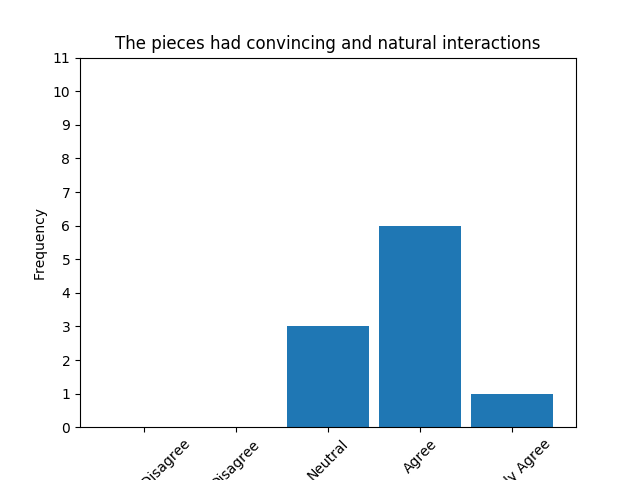
\includegraphics[width=\textwidth]{images/questions/13}
\end{subfigure}
\begin{subfigure}{.5\textwidth}
    \centering
    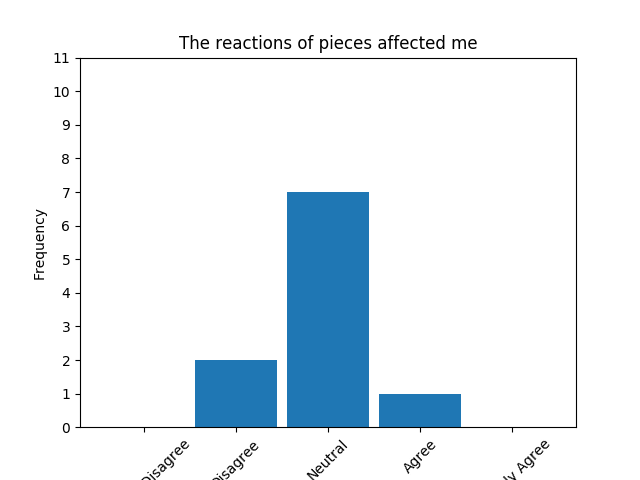
\includegraphics[width=\textwidth]{images/questions/14}
\end{subfigure}%
\begin{subfigure}{.5\textwidth}
    \centering
    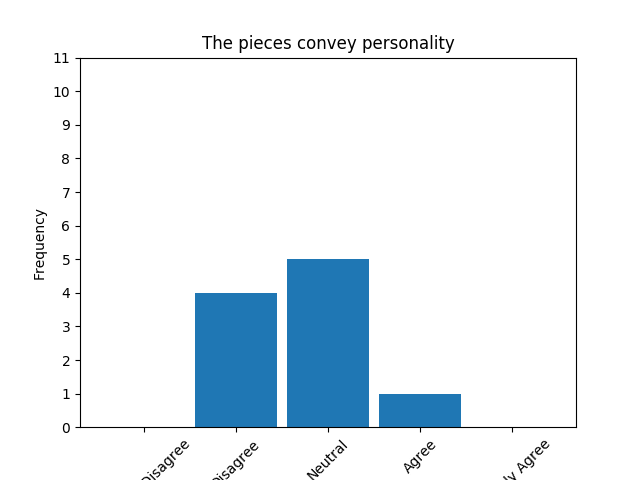
\includegraphics[width=\textwidth]{images/questions/15}
\end{subfigure}
\caption[short]{Questions 9-16 in Questionnaire}\label{fig:qmiddel}
\end{figure}

\begin{figure}[!ht]
\centering
\begin{subfigure}{.5\textwidth}
    \centering
    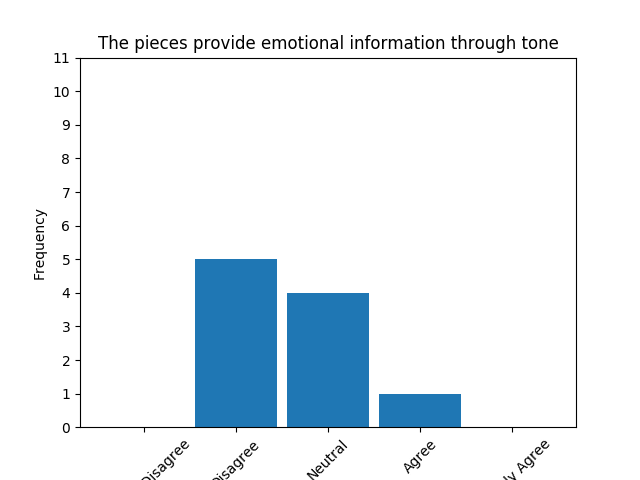
\includegraphics[width=\textwidth]{images/questions/16}
\end{subfigure}%
\begin{subfigure}{.5\textwidth}
    \centering
    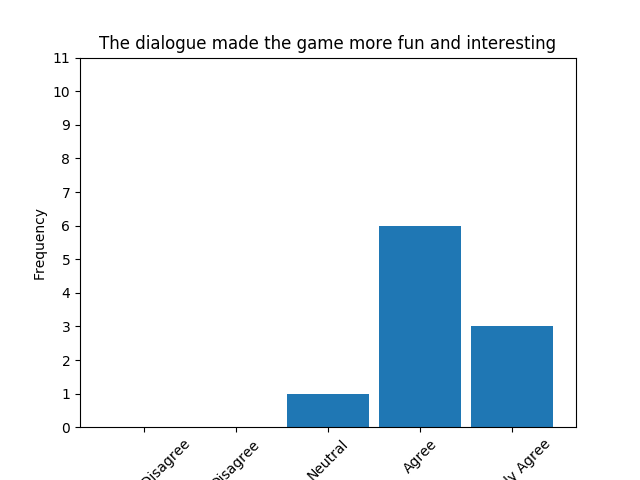
\includegraphics[width=\textwidth]{images/questions/17}
\end{subfigure}
\caption[short]{Questions 17 and 18 in Questionnaire} \label{fig:qlast}
\end{figure}

Unfortunately the popularity of chess meant that only one of our participants had not played in either a very long time or never at all. The results mostly lean to the negative side, but only slightly, and there are some cases were participants were impressed.

A majority of players said they lost track of time while playing. Without being able to compare results with chess without dialogues, it is difficult to state the cause of this. It is possible that the conversations provide enough of a narrative to make players lose focus on time. 

The game also ranked highly for the question "Playing makes me feel calm". This was expected, as gameplay is mostly reading the dialogue without much other stimulation.

In regards to the emotional response to the agents and the game, the results of the questions "I feel different" and "I get wound up" vary wildly. Players were definitely not 'wound up' or agitated by the game, which suggests that the player directed insults were ineffective or that the challenge was not sufficient for most players.

The linguistic accuracy of the pieces were rated highly. However, some of the freetext comments mentioned that the justifications all sounded the same, and another comment did suggest that the dialogue was not perfectly fluid. These issues could be resolved through careful tailoring of the BNF grammars used. The original interface for values only provided a single string representation for each of the opinions when evaluating the response to a move, and so this comment highlighted the need for the values to be included in the grammars to increase the number of wordings used.

The conversation planning seemed to be successful given the majority of players agreeing with the statement "The pieces had convincing and natural interactions". Given this was likely the part of the project that had taken the most time, it was rewarding to receive such a positive response.

Piece reactions did not seem to have much of an effect on players with the majority of participants giving a neutral response. One of the comments mentioned the reactions seeming random, which could point to issues with conveying personality of the agents, or a lack of emotion in the generated text. This is further evidenced by the replies to the final question, where most players did not seem to get a sense of personality from each of the pieces.

One of the reasons given for this in the comments were that maybe more exposure to the pieces were required to make the personalities recognisable, and another highlighted the problem that the similar appearance of the pieces made it difficult to track who said what and therefore remember which piece showed which personality traits. The nametags were implemented to avoid this issue, but clearly another solution is necessary to make each piece more unique.

Another interesting comment was that the phrases spoken by pieces would sometimes appear too long which ruined the flow of conversation slightly. The participant suggested breaking up longer statements by placing a limit on the length of each piece of dialogue, and splitting any statements that overflowed this limit. All the participants did enjoy the novelty of the concept however, which definitely suggested that these conversational agents would worth investigating further.

While continuing to play, one participant pointed out that it was hard to say if a piece had been 'convinced' to make a move, as the movement often seemed to come out of nowhere, even if it was the move currently being convinced. It is difficult to determine what change needed to be made to remedy this issue, but doing so would be likely to provide more satisfying gameplay. Further play also allowed some participants to begin to spot patterns and repetition in speech, which made it clear that the corpus of statements needed to be made larger. 

Given one of the goals were to make the agent interactions humourous, participants were observed while playing to see if a smile or a laugh was given in reaction to agent behaviour. Fortunately, this did occur when agents caught the human player off guard by insulting their moves, or insulting each other. 

\subsection{Improvements}

Due to time constraints, only some of the issues raised were able to be attacked before the final artefact had to be submitted.

The test coverage was greatly improved to try catch edge cases were the conversation planner would fail. The grammars used by each personality were also extended to try create more variation in the phrases produced during a game.

\section{Future Work}

The user feedback suggested that though this implementation was far from perfect, the conversational agents were an interesting novelty that is worth exploring further. Many improvements to our own work have already been discussed, but other extensions exist that would improve conversational agents.

With more time, a more thorough study that would compare player enjoyment with dialogue disabled and then enabled would shed more light on the benefits of the conversational agents. If we were able to make those who dislike chess or have not played before consider the game again, or provide a novel experience for those who enjoy the game already, then the project could definitely be deemed a success.

Other work that would definitely improve the current implementation would be accounting for piece value when choosing moves and using typical chess AI approaches such as minmax searches to make the chosen moves slightly more strategic.

The need to manually craft the grammars for agents is clearly a severely limiting factor for how an implementation like this could scale. Since any game wanting to include natural language generation will likely also require special domain knowledge to be accounted for, its unlikely a public database could be used. If the goal was to simply make conversational background characters for the sake of creating realism however, our approach could be useful.

Unfortunately, chat bots been used to perform social engineering for unethical reasons. Conversational chatbots could be used for propaganda purposes for emulating real people on social networks to try and fake popularity of certain topics or spread lies. \cite{conveval} refer to one case where a chatbot was convincing enough for someone to think it was romantically interested in them. Agents that are able to create this level of realistic conversation could also be used to help identify when it is occurring, and simply researching how these agents could operate will help us identify patterns that such bots might follow.

\section{Conclusion}

By referring to the original project goals which - due to the wide range of topics being covered by this project - were definitely ambitious, it is clear that this project has been fairly successful.  All of the primary goals set were met fully, all of the secondary goals were either partially or fully implemented, and the tertiary goal of a detailed graphical interface was attempted. User feedback definitely highlighted the need for improvements to the graphical interface for the game.

Researching this project was a fantastic opportunity to learn more about multiagent systems, natural language generation, and social artificial intelligence. Whilst progress definitely suffered due to the wrong approaches being taken early on in development for certain aspects of the if the project, the final product was able to include each of these topics to some degree. 

Gathering user feedback was rewarding, and the constructive criticism given provided a clear guide of what work would be required to bring this project to its full potential, but I am nonetheless proud of what has been produced.

\section{Acknowledgements}

I would like to thank my supervisors: Dr Alice Toniolo for her expert advice and support throughout the project and helping set realistic but still ambitious goals at each step of the way, and Christopher Stone for providing excellent guidance to help me understand and implement the natural language generation approaches used in industry and those adopted within this project. Your shared enthusiasm for the resulting project was thoroughly appreciated.

I would also like to thank my fellow students for helping by taking part in the user feedback exercises, as well as providing great company during the development of the project.

Finally, I would also like to thank my family for getting me through the final stretch of work needed. 


\bibliographystyle{unsrt}
\bibliography{mybib}

\section{Appendix}

% TODO include testing description, user manual, and ethics forms in appendix
\subsection{Testing Summary}
\subsection{User Manual}
\subsection{Ethics}

\vspace{12pt}

\end{document}

